\begin{exercice*}
    \begin{enumerate}
        \item Construire un triangle $A'B'C'$ isométrique au triangle $ABC$ en utilisant le côté $[A'B']$.
        \par\smallskip Il y a deux solutions à tracer avec des couleurs distinctes.
        \item Faire un commentaire sur ces deux solutions.
    \end{enumerate}    
    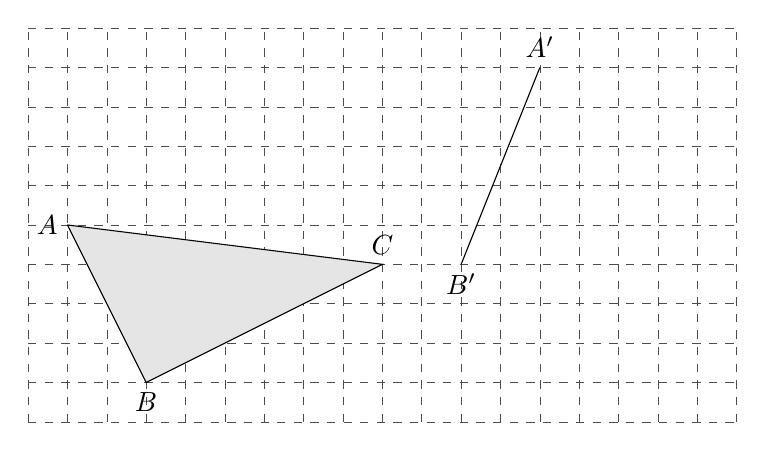
\begin{tikzpicture}[scale = 0.5]
        \draw[help lines, color=black!70, dashed] (0,0) grid (18,10);
        \coordinate[label=left:$A$] (A) at (1,5);
        \coordinate[label=below:$B$] (B) at (3,1);
        \coordinate[label=above:$C$] (C) at (9,4);
        \coordinate[label=above:$A'$] (A') at (13,9);
        \coordinate[label=below:$B'$] (B') at (11,4);            
        \draw[fill=gray!20] (A) -- (B) -- (C) -- (A);
        \draw (A') -- (B');
    \end{tikzpicture}
\end{exercice*}
\begin{corrige}
    %\setcounter{partie}{0} % Pour s'assurer que le compteur de \partie est à zéro dans les corrigés
    \phantom{rrr}    

    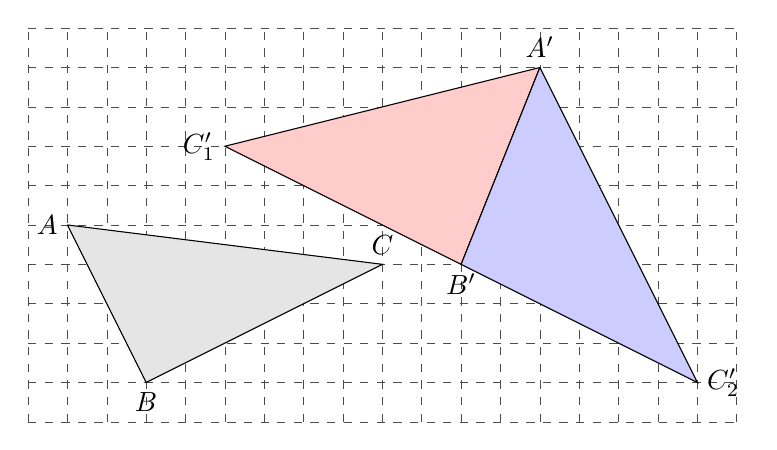
\begin{tikzpicture}[scale = 0.5]
        \draw[help lines, color=black!70, dashed] (0,0) grid (18,10);
        \coordinate[label=left:$A$] (A) at (1,5);
        \coordinate[label=below:$B$] (B) at (3,1);
        \coordinate[label=above:$C$] (C) at (9,4);
        \coordinate[label=above:$A'$] (A') at (13,9);
        \coordinate[label=below:$B'$] (B') at (11,4);            
        \coordinate[label=left:$C_{1}'$] (C1) at (5,7);
        \coordinate[label=right:$C_{2}'$] (C2) at (17,1);        
        \draw[fill=gray!20] (A) -- (B) -- (C) -- (A);
        \draw[fill=red!20] (A') -- (B') -- (C1) -- (A');
        \draw[fill=blue!20] (A') -- (B') -- (C2) -- (A');

    \end{tikzpicture}
\end{corrige}

